\section{O‘zgaruvchan tok zanjirida aktiv  qarshilik, kondensator va induktiv g‘altak. }


\begin{enumerate}

\item O‘zgaruvchan tok manbaiga rezistor, kondensator va g‘altak ketma-ket ulandi. Kuchlanish tebranishlarining amplitudasi rezistorda $4$ V ga, kondensatorda $6$ V ga, g‘altakda esa $3$ V ga teng. Manba qisqichlaridagi kuchlanish tebranishlarining amplitudasi necha Volt?
\begin{enumerate}[label=\Alph*)]
\item 6.
\item 4.
\item 5.
\item 3.
\item TJY.
\end{enumerate}

\item O‘zgaruvchan tok zanjiriga induktiv g‘altak, kondensator va rezistor ketma-ket ulangan. G‘altak, kondensator va rezistor uchlaridagi kuchlanishlar mos ravishda $30$ V, $24$ V va $8$ V. Zanjirdagi umumiy kuchlanish qanday (V)?
\begin{enumerate}[label=\Alph*)]
\item 10.
\item 14.
\item 21.
\item 46.
\item 62.
\end{enumerate}

\item O‘zgaruvchan tok zanjiriga rezistor va kondensator ketma-ket ulangan. Rezistorga ulangan voltmetr $60$ V ni, kondensator uchlariga ulangan voltmetr $80$ V ni ko‘rsatsa, tarmoqdagi umumiy kuchlanish necha V?
\begin{enumerate}[label=\Alph*)]
\item 20.
\item 60.
\item 80.
\item 100.
\item 140.
\end{enumerate}

\item Rasmda ko‘rsatilgan zanjirdagi kuchlanishlar $U_L=80$ V, $U_C=60$ V bo‘lsa, $U$ necha Volt bo‘ladi?

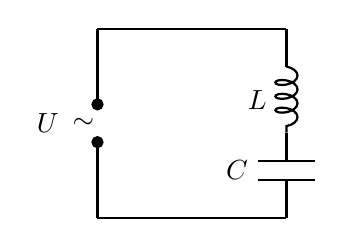
\begin{tikzpicture}[thick, scale=1.2]
    % Manba (AC Source)
    \draw (0, 0.8) -- (0, 0);
    \draw (0, 1.2) -- (0, 2);
    \filldraw (0, 0.8) circle (1.5pt);
    \filldraw (0, 1.2) circle (1.5pt);
    \node at (-0.15, 1) {$\sim$};
    \node[left] at (-0.3, 1) {$U$};

    % Zanjir simlari
    \draw (0, 2) -- (2, 2);
    \draw (0, 0) -- (2, 0);

    % G'altak (L) - yuqoriroqda
    \draw (2, 2) -- (2, 1.6);
    \draw[decoration={coil, aspect=0.5, segment length=5pt, amplitude=4pt}, decorate] (2, 1.6) -- (2, 0.9);
    \node[left] at (1.9, 1.25) {$L$};

    % Kondensator (C) - pastroqda
    \draw (2, 0.9) -- (2, 0.6);
    \draw (1.7, 0.6) -- (2.3, 0.6);
    \draw (1.7, 0.4) -- (2.3, 0.4);
    \draw (2, 0.4) -- (2, 0);
    \node[left] at (1.7, 0.5) {$C$};

\end{tikzpicture}

\begin{enumerate}[label=\Alph*)]
\item 100.
\item 140.
\item $\sqrt{140}$.
\item 20.
\item 10.
\end{enumerate}

\item O‘zgaruvchan tok zanjiriga induktiv g‘altak va kondensator ketma-ket ulangan. Induktiv g‘altakka ulangan voltmetr $400$ V ni, kondensatorga ulangan voltmetr $180$ V ni ko‘rsatib turibdi. Tarmoqdagi umumiy kuchlanish qanday (V)?
\begin{enumerate}[label=\Alph*)]
\item 180.
\item 220.
\item 290.
\item 400.
\item 580.
\end{enumerate}

\item Aktiv qarshilik va induktivlik g‘altagi o‘zgaruvchan tok manbaiga ketma-ket ulangan. AB nuqtalar orasidagi potensiallar farqi $40$ V, BC nuqtalar orasidagi potensiallar farqi $30$ V ga teng bo‘lsa, AC nuqtalar orasidagi potensiallar farqi necha V ga teng (V)?

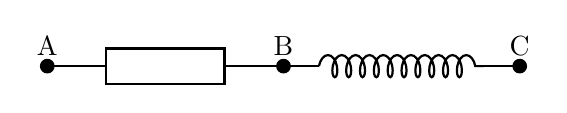
\begin{tikzpicture}[thick, scale=1.5]
    % Nuqtalar (A, B, C)
    \filldraw (0,0) circle (1.5pt) node[above] {A};
    \filldraw (2,0) circle (1.5pt) node[above] {B};
    \filldraw (4,0) circle (1.5pt) node[above] {C};

    % Simlar va elementlar
    \draw (0,0) -- (0.5,0);
    
    % Rezistor (A va B orasida)
    \draw (0.5,-0.15) rectangle (1.5,0.15);
    \draw (1.5,0) -- (2,0);
    
    % G'altak (B va C orasida)
    \draw (2,0) -- (2.3,0);
    \draw[decoration={coil, aspect=0.5, segment length=5pt, amplitude=4pt}, decorate] (2.3,0) -- (3.7,0);
    \draw (3.7,0) -- (4,0);

\end{tikzpicture}

\begin{enumerate}[label=\Alph*)]
\item 70.
\item 10.
\item 50.
\item 60.
\item 5.
\end{enumerate}

\item Zanjir ketma-ket ulangan $24~\Omega$ aktiv, $30~\Omega$ sig‘im va $30~\Omega$ induktiv qarshilikdan iborat. Zanjirning to‘la qarshiligini toping ($\Omega$).
\begin{enumerate}[label=\Alph*)]
\item 84.
\item 65.
\item 54.
\item 30.
\item 24.
\end{enumerate}

\item O‘zgaruvchan tok zanjiriga qarshiligi $70~\Omega$ bo‘lgan rezistor, sig‘imi $6~\Omega$ bo‘lgan kondensator, induktivligi $30~\Omega$ bo‘lgan g‘altak ketma-ket ulangan. Zanjirning to‘la qarshiligini qanday ($\Omega$)?
\begin{enumerate}[label=\Alph*)]
\item 65.
\item 53.
\item 95.
\item 74.
\item 109.
\end{enumerate}

\item Siklik (doiraviy) chastotasi $1000$ rad/s bo‘lgan o‘zgaruvchan tok zanjiriga induktivligi $2$ H bo‘lgan g‘altak va sig‘imi $1~\mu$F bo‘lgan kondensator ketma-ket ulangan. Zanjirning to‘la qarshiligini toping (k$\Omega$).
\begin{enumerate}[label=\Alph*)]
\item 1.
\item 3.
\item 10.
\item 30.
\item 100.
\end{enumerate}

\item Tok zanjiriga induktivligi $31,4$ H bo‘lgan g‘altak va $314$ nF sig‘imli kondensator ketma-ket ulangan. O‘zgaruvchan tok chastotasi $50$ Hz bo‘lsa, zanjirning to‘la qarshiligi ($\Omega$) nimaga teng bo‘ladi? Tutashtiruvchi simlarning qarshiligini hisobga olmang. $\pi^2\approx10$.
\begin{enumerate}[label=\Alph*)]
\item 0.
\item 1.
\item 3,14.
\item 6,28.
\item 10.
\end{enumerate}

\item O‘zgaruvchan tok manbayiga qarshiligi $8~\text{k}\Omega$ bo‘lgan aktiv qarshilik va induktivligi $20$ H bo‘lgan induktiv g‘altak ketma-ket ulangan. Agar o‘zgaruvchan tokning chastotasi $50$ Hz bo‘lsa, zanjirning to‘la qarshiligini (k$\Omega$) aniqlang. $\pi=3$.
\begin{enumerate}[label=\Alph*)]
\item 10.
\item 6.
\item 8.
\item 12.
\item 5.
\end{enumerate}

\item Quyida keltirilgan o‘zgaruvchan tok zanjirining to‘la qarshiligi $Z=3\sqrt5~\Omega$ ga teng. $R_1=12~\Omega$, $X_L=10~\Omega$ va $X_C=4~\Omega$ bo‘lsa, $R_2$ nimaga teng($\Omega$)?

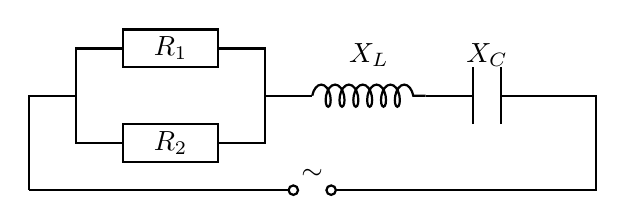
\begin{tikzpicture}[thick, scale=1.2]
    % Asosiy kontur ramkasi
    \draw (0,0) -- (0,1) -- (0.5,1);
    \draw (0,0) -- (2.76,0);
    \draw (3.24,0)--(6,0) -- (6,1) -- (5.5,1);

    % Parallel qism (R1 va R2)
    \draw (0.5, 1) -- (0.5, 1.5) -- (1, 1.5);
    \draw (0.5, 1) -- (0.5, 0.5) -- (1, 0.5);
    
    \draw (1, 1.3) rectangle (2, 1.7) node[midway] {$R_1$};
    \draw (1, 0.3) rectangle (2, 0.7) node[midway] {$R_2$};
    
    \draw (2, 1.5) -- (2.5, 1.5) -- (2.5, 1);
    \draw (2, 0.5) -- (2.5, 0.5) -- (2.5, 1);
    
    % Induktivlik g'altagi (XL)
    \draw (2.5, 1) -- (3, 1);
    \draw[decoration={coil, aspect=0.5, segment length=5pt, amplitude=4pt}, decorate] (3, 1) -- (4.2, 1);
    \node[above] at (3.6, 1.2) {$X_L$};

    % Kondensator (XC)
    \draw (4.2, 1) -- (4.7, 1);
    \draw (4.7, 0.7) -- (4.7, 1.3);
    \draw (5, 0.7) -- (5, 1.3);
    \draw (5, 1) -- (5.5, 1);
    \node[above] at (4.85, 1.2) {$X_C$};

    % O'zgaruvchan tok manbai (Pastda)
    \draw (2.8, 0) circle (0.05);
    \draw (3.2, 0) circle (0.05);
    \node[above] at (3, 0) {$\sim$};

\end{tikzpicture}

\begin{enumerate}[label=\Alph*)]
\item 4.
\item 8.
\item 12.
\item 16.
\item 6.
\end{enumerate}

\item Sig‘imi $100~\mu$F bo‘lgan kondensator, induktivligi $200$ mH bo‘lgan g‘altak va qarshiligi $60~\Omega$ bo‘lgan reostat ketma-ket ulangan zanjirdagi tokning o‘zgarish qonuni $i=8\sin100t$ ko‘rinishga ega. Zanjirning to‘la qarshiligi necha $\Omega$?
\begin{enumerate}[label=\Alph*)]
\item 640.
\item 360.
\item 6400.
\item 80.
\item 100.
\end{enumerate}

\item Siklik (doiraviy) chastotasi $300$ rad/s bo‘lgan o‘zgaruvchan tok zanjiriga $4~\Omega$ qarshilikka ega rezistor va induktivligi $10$ mH bo‘lgan g‘altak ketma-ket ulangan. Zanjirdan o‘tayotgan tok kuchi amplitudasi $50$ A ga teng bo‘lsa, zanjir uchlaridagi kuchlanish amplitudasi qanday (V)?
\begin{enumerate}[label=\Alph*)]
\item 200.
\item 250.
\item 350.
\item 400.
\item 500.
\end{enumerate}

\item O‘zgaruvchan tok zanjirining aktiv qarshiligi $16~\Omega$, reaktiv qarshiligi $12~\Omega$. Zanjir quvvat koeffitsiyenti nimaga teng?
\begin{enumerate}[label=\Alph*)]
\item 0,6.
\item 0,64.
\item 0,92.
\item 0,8.
\item 0.
\end{enumerate}

\item Zanjirning aktiv qarshiligi $7~\Omega$, reaktiv qarshiligi $24~\Omega$. Zanjir uchun quvvat koeffitsiyenti nimaga teng?
\begin{enumerate}[label=\Alph*)]
\item 0,28.
\item 0,6.
\item 0,64.
\item 0,92.
\item 0,3.
\end{enumerate}

\item Siklik (doiraviy) chastotasi $10^3$ rad/s bo‘lgan o‘zgaruvchan tok zanjiriga qarshiligi $15~\Omega$ bo‘lgan rezistor va induktivligi $0,02$ H bo‘lgan g‘altak ketma-ket ulangan. Agar zanjirdagi to‘la kuchlanish amplituda qiymati $1$ kV bo‘lsa, tok kuchining amplitudasi qanday (A)?
\begin{enumerate}[label=\Alph*)]
\item 5.
\item 35.
\item 40.
\item 70.
\item 80.
\end{enumerate}

\item O‘zgaruvchan tok zanjiriga sig‘im qarshiligi $10~\Omega$ bo‘lgan kondensator va induktiv qarshiligi $20~\Omega$ bo‘lgan g‘altak ketma-ket ulangan. Agar tokning samarador (effektiv) qiymati $2$ A bo‘lsa, zanjir uchlaridagi kuchlanishning samarali qiymati qanday (V)?
\begin{enumerate}[label=\Alph*)]
\item 60.
\item 43.
\item 40.
\item 30.
\item 20.
\end{enumerate}

\item Siklik (doiraviy) chastotasi $10^4$ rad/s bo‘lgan o‘zgaruvchan tok zanjiriga qarshiligi $100~\Omega$ bo‘lgan rezistor va sig‘imi $1~\mu$F bo‘lgan kondensator ketma-ket ulangan. Zanjirdagi tashqi kuchlanish amplitudasi $300$ V. Zanjirdan o‘tayotgan tok kuchi amplitudasi qanday (A)?
\begin{enumerate}[label=\Alph*)]
\item 6.
\item 4,2.
\item 3.
\item 2,1.
\item 1,5.
\end{enumerate}

\item O‘zgaruvchan tok zanjiriga aktiv qarshiligi $10~\Omega$ bo‘lgan rezistor, induktiv qarshiligi $20~\Omega$ bo‘lgan g‘altak va sig‘im qarshiligi $30~\Omega$ bo‘lgan kondensator ketma-ket ulangan. Agar o‘zgaruvchan tok kuchlanishining amplituda qiymati $200$ V bo‘lsa, tok kuchining amplitudasi qanday (A)?
\begin{enumerate}[label=\Alph*)]
\item 1,4.
\item 2.
\item 3,3.
\item 14.
\item 20.
\end{enumerate}

\item Zanjir ketma-ket ulangan $9~\Omega$ aktiv va $12~\Omega$ induktiv qarshilikdan tuzilgan. Tok bilan kuchlanish tebranishlari orasidagi faza siljishining kosinusi qanday?
\begin{enumerate}[label=\Alph*)]
\item 0.
\item 0,3.
\item 0,6.
\item 0,8.
\item 1.
\end{enumerate}

\item Zanjir ketma-ket ulangan $18~\Omega$ aktiv qarshilik va $24~\Omega$ sig‘im qarshilikdan tuzilgan. Tok bilan kuchlanish tebranishlari orasidagi faza siljishining kosinusini toping.
\begin{enumerate}[label=\Alph*)]
\item $1/2$.
\item 0,6.
\item $\sqrt2/2$.
\item $\sqrt3/2$.
\item 1.
\end{enumerate}

\item Ushbu elektr zanjiridagi tok kuchining effektiv qiymatini toping(A).

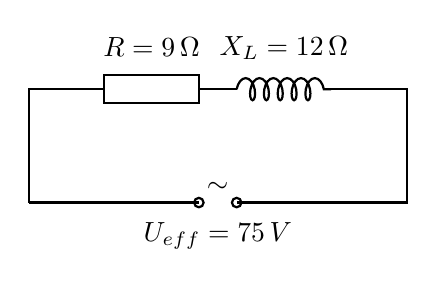
\begin{tikzpicture}[thick, scale=1.2]
    % Zanjir ramkasi
    \draw (0,0) -- (0,1.2) -- (0.8,1.2);
    \draw (1.8,1.2) -- (2.2,1.2);
    \draw (3.2,1.2) -- (4,1.2) -- (4,0) -- (2.2,0);
    \draw (1.8,0) -- (0,0);

    % Rezistor (R = 9 Ohm)
    \draw (0.8, 1.05) rectangle (1.8, 1.35) node[midway, above=8pt] {$R=9 \, \Omega$};

    % Induktivlik g'altagi (XL = 12 Ohm)
    \draw[decoration={coil, aspect=0.5, segment length=5pt, amplitude=4pt}, decorate] (2.2, 1.2) -- (3.2, 1.2);
    \node[above] at (2.7, 1.4) {$X_L=12 \, \Omega$};

    % O'zgaruvchan tok manbai (Ueff = 75 V)
    \draw (1.8, 0) circle (0.05);
    \draw (2.2, 0) circle (0.05);
    \node[above] at (2, 0) {$\sim$};
    \node[below] at (2, -0.1) {$U_{\text{eff}}=75 \, \text{V}$};

\end{tikzpicture}

\begin{enumerate}[label=\Alph*)]
\item 1.
\item 2.
\item 3.
\item 4.
\item 5.
\end{enumerate}

\item Ushbu elektr zanjiridagi quvvat koeffitsienti ($\cos\Delta\varphi$) ni toping.

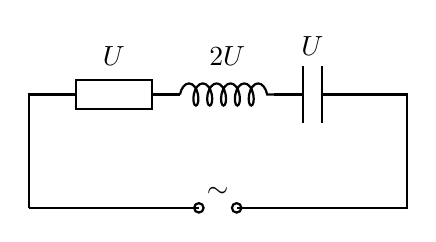
\begin{tikzpicture}[thick, scale=1.2]
    % Zanjir asosiy simlari
    \draw (0,0) -- (0,1.2) -- (0.5,1.2);
    \draw (3.5,1.2) -- (4,1.2) -- (4,0) -- (2.2,0);
    \draw (1.8,0) -- (0,0);

    % Rezistor (Kuchlanish U)
    \draw (0.5, 1.05) rectangle (1.3, 1.35);
    \node[above] at (0.9, 1.4) {$U$};
    \draw (1.3, 1.2) -- (1.6, 1.2);

    % G'altak (Kuchlanish 2U)
    \draw[decoration={coil, aspect=0.5, segment length=5pt, amplitude=4pt}, decorate] (1.6, 1.2) -- (2.6, 1.2);
    \node[above] at (2.1, 1.4) {$2U$};
    \draw (2.6, 1.2) -- (2.9, 1.2);

    % Kondensator (Kuchlanish U)
    \draw (2.9, 0.9) -- (2.9, 1.5);
    \draw (3.1, 0.9) -- (3.1, 1.5);
    \node[above] at (3, 1.5) {$U$};
    \draw (3.1, 1.2) -- (3.5, 1.2);

    % O'zgaruvchan tok manbai
    \draw (1.8, 0) circle (0.05);
    \draw (2.2, 0) circle (0.05);
    \node[above] at (2, 0) {$\sim$};

\end{tikzpicture}

\begin{enumerate}[label=\Alph*)]
\item $1/2$.
\item $3/5$.
\item $2/3$.
\item $\sqrt2/2$.
\item $4/5$.
\end{enumerate}

\item Ushbu 2 ta rasmli elektr zanjirlarda quvvat koeffitsienti bir xil. Ikkala zanjirdagi tok kuchlarining effektiv qiymatlari nisbati $I_1/I_2$ ni toping.

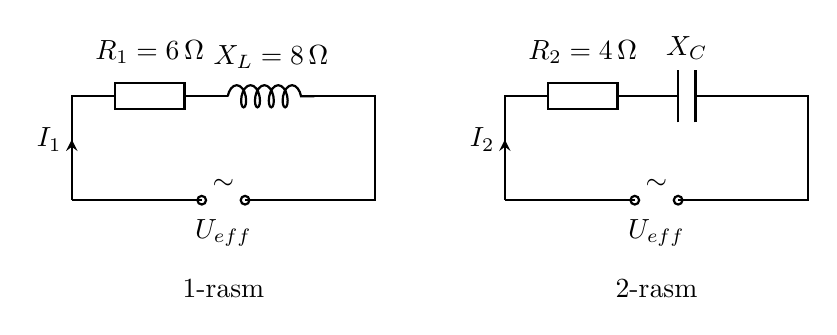
\begin{tikzpicture}[thick, scale=1.1]

    % --- 1-rasm (Rezistor va G'altak) ---
    \begin{scope}[xshift=0cm]
        \draw (0,0) -- (0,1.2) -- (0.5,1.2);
        \draw (1.3,1.2) -- (1.8,1.2);
        \draw (2.8,1.2) -- (3.5,1.2) -- (3.5,0) -- (2,0);
        \draw (1.5,0) -- (0,0);

        % Rezistor R1=6 Ohm
        \draw (0.5, 1.05) rectangle (1.3, 1.35) node[midway, above=8pt] {$R_1=6 \, \Omega$};
        
        % G'altak XL=8 Ohm
        \draw[decoration={coil, aspect=0.5, segment length=5pt, amplitude=4pt}, decorate] (1.8, 1.2) -- (2.8, 1.2);
        \node[above] at (2.3, 1.4) {$X_L=8 \, \Omega$};

        % Tok yo'nalishi I1
        \draw[->, >=stealth] (0, 0.5) -- (0, 0.7) node[left] {$I_1$};

        % Manba Ueff
        \draw (1.5, 0) circle (0.05);
        \draw (2, 0) circle (0.05);
        \node[above] at (1.75, 0) {$\sim$};
        \node[below] at (1.75, -0.1) {$U_{\text{eff}}$};
        
        \node[below] at (1.75, -0.8) {1-rasm};
    \end{scope}

    % --- 2-rasm (Rezistor va Kondensator) ---
    \begin{scope}[xshift=5cm]
        \draw (0,0) -- (0,1.2) -- (0.5,1.2);
        \draw (1.3,1.2) -- (2,1.2);
        \draw (2.2,1.2) -- (3.5,1.2) -- (3.5,0) -- (2,0);
        \draw (1.5,0) -- (0,0);

        % Rezistor R2=4 Ohm
        \draw (0.5, 1.05) rectangle (1.3, 1.35) node[midway, above=8pt] {$R_2=4 \, \Omega$};
        
        % Kondensator XC
        \draw (2, 0.9) -- (2, 1.5);
        \draw (2.2, 0.9) -- (2.2, 1.5);
        \node[above] at (2.1, 1.5) {$X_C$};

        % Tok yo'nalishi I2
        \draw[->, >=stealth] (0, 0.5) -- (0, 0.7) node[left] {$I_2$};

        % Manba Ueff
        \draw (1.5, 0) circle (0.05);
        \draw (2, 0) circle (0.05);
        \node[above] at (1.75, 0) {$\sim$};
        \node[below] at (1.75, -0.1) {$U_{\text{eff}}$};
        
        \node[below] at (1.75, -0.8) {2-rasm};
    \end{scope}

\end{tikzpicture}

\begin{enumerate}[label=\Alph*)]
\item $1/2$.
\item $1/3$.
\item $2/3$.
\item $1$.
\item $4/5$.
\end{enumerate}

\item Ushbu elektr zanjiridagi kuchlanish 
$u=U\sin\omega t$, tok kuchi esa 
$i=I\sin\left(\omega t-\dfrac{\pi}{6}\right)$ 
qonun bo‘yicha o‘zgaradi. Zanjirdagi induktiv qarshilikni ($X_L$) toping($\Omega$).

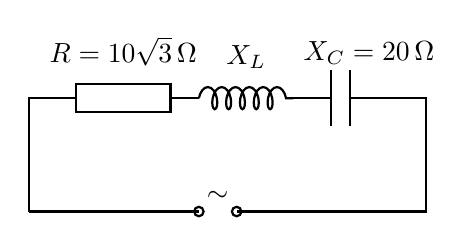
\begin{tikzpicture}[thick, scale=1.2]
    % Zanjir asosiy simlari
    \draw (0,0) -- (0,1.2) -- (0.5,1.2);
    \draw (3.8,1.2) -- (4.2,1.2) -- (4.2,0) -- (2.2,0);
    \draw (1.8,0) -- (0,0);

    % Rezistor (R = 10*sqrt(3) Ohm)
    \draw (0.5, 1.05) rectangle (1.5, 1.35) node[midway, above=8pt] {$R=10\sqrt{3} \, \Omega$};
    \draw (1.5, 1.2) -- (1.8, 1.2);

    % G'altak (XL)
    \draw[decoration={coil, aspect=0.5, segment length=5pt, amplitude=4pt}, decorate] (1.8, 1.2) -- (2.8, 1.2);
    \node[above] at (2.3, 1.4) {$X_L$};
    \draw (2.8, 1.2) -- (3.2, 1.2);

    % Kondensator (XC = 20 Ohm)
    \draw (3.2, 0.9) -- (3.2, 1.5);
    \draw (3.4, 0.9) -- (3.4, 1.5);
    \node[above] at (3.6, 1.45) {$X_C=20 \, \Omega$};
    \draw (3.4, 1.2) -- (3.8, 1.2);

    % O'zgaruvchan tok manbai
    \draw (1.8, 0) circle (0.05);
    \draw (2.2, 0) circle (0.05);
    \node[above] at (2, 0) {$\sim$};

\end{tikzpicture}

\begin{enumerate}[label=\Alph*)]
\item 5.
\item 15.
\item 20.
\item 25.
\item 30.
\end{enumerate}

\item Ushbu elektr zanjiridagi kuchlanish 
$u=U\sin\omega t$, tok kuchi esa 
$i=10\sqrt2\sin\left(50t+\dfrac{\pi}{3}\right)$ 
qonun bo‘yicha o‘zgaradi. Zanjirdagi kuchlanishning effektiv qiymatini toping(V). $[u]=$Volt, $[i]=$Amper.

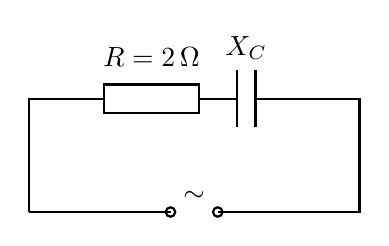
\begin{tikzpicture}[thick, scale=1.2]
    % Zanjir asosiy simlari
    \draw (0,0) -- (0,1.2) -- (0.8,1.2);
    \draw (1.8,1.2) -- (2.2,1.2);
    \draw (2.4,1.2) -- (3.5,1.2) -- (3.5,0) -- (2,0);
    \draw (1.5,0) -- (0,0);

    % Rezistor (R = 2 Ohm)
    \draw (0.8, 1.05) rectangle (1.8, 1.35) node[midway, above=8pt] {$R=2 \, \Omega$};

    % Kondensator (XC)
    \draw (2.2, 0.9) -- (2.2, 1.5);
    \draw (2.4, 0.9) -- (2.4, 1.5);
    \node[above] at (2.3, 1.5) {$X_C$};

    % O'zgaruvchan tok manbai
    \draw (1.5, 0) circle (0.05);
    \draw (2, 0) circle (0.05);
    \node[above] at (1.75, 0) {$\sim$};

\end{tikzpicture}

\begin{enumerate}[label=\Alph*)]
\item 20.
\item $20\sqrt3$.
\item 40.
\item $40\sqrt3$.
\item 80.
\end{enumerate}

\item Ushbu elektr zanjiridagi tok kuchining effektiv qiymatini toping(A).

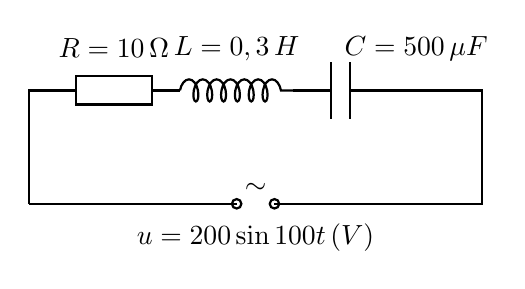
\begin{tikzpicture}[thick, scale=1.2]
    % Zanjir asosiy simlari
    \draw (0,0) -- (0,1.2) -- (0.5,1.2);
    \draw (4,1.2) -- (4.8,1.2) -- (4.8,0) -- (2.6,0);
    \draw (2.2,0) -- (0,0);

    % Rezistor (R = 10 Ohm)
    \draw (0.5, 1.05) rectangle (1.3, 1.35) node[midway, above=8pt] {$R=10 \, \Omega$};
    \draw (1.3, 1.2) -- (1.6, 1.2);

    % G'altak (L = 0,3 H)
    \draw[decoration={coil, aspect=0.5, segment length=5pt, amplitude=4pt}, decorate] (1.6, 1.2) -- (2.8, 1.2);
    \node[above] at (2.2, 1.4) {$L=0,3 \, \text{H}$};
    \draw (2.8, 1.2) -- (3.2, 1.2);

    % Kondensator (C = 500 uF)
    \draw (3.2, 0.9) -- (3.2, 1.5);
    \draw (3.4, 0.9) -- (3.4, 1.5);
    \node[above] at (4.1, 1.4) {$C=500 \, \mu\text{F}$};
    \draw (3.4, 1.2) -- (4, 1.2);

    % O'zgaruvchan tok manbai
    \draw (2.2, 0) circle (0.05);
    \draw (2.6, 0) circle (0.05);
    \node[above] at (2.4, 0) {$\sim$};
    \node[below] at (2.4, -0.1) {$u = 200 \sin 100t \, (\text{V})$};

\end{tikzpicture}

\begin{enumerate}[label=\Alph*)]
\item 5.
\item $10\sqrt2$.
\item 10.
\item $20\sqrt2$.
\item 20.
\end{enumerate}

\item Quyidagi zanjirning to‘la qarshilik vektori 2-rasmda ko‘rsatilgandek. Kondensatordagi kuchlanish tushuvining effektiv qiymatini toping(V). $\sin53^0=0,8$, $\cos53^0=0,6$.

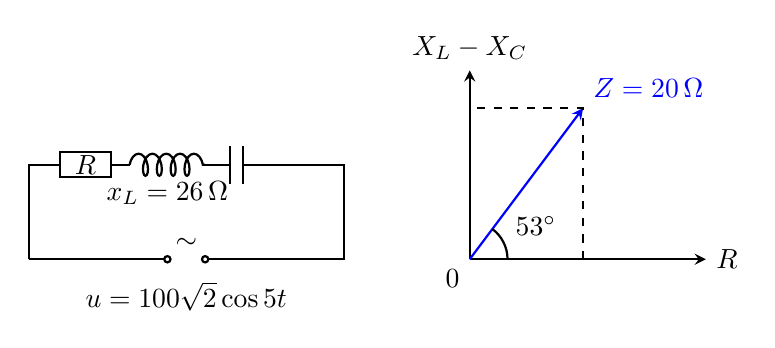
\begin{tikzpicture}[thick, scale=0.8]

    % --- 1-qism: Elektr zanjiri sxemasi ---
    \begin{scope}[xshift=0cm]
        % Zanjir simlari
        \draw (0,0) -- (0,1.5) -- (0.5,1.5);
        \draw (4,1.5) -- (5,1.5) -- (5,0) -- (2.83,0);
        \draw (2.17,0) -- (0,0);

        % Rezistor R
        \draw (0.5, 1.3) rectangle (1.3, 1.7) node[midway] {$R$};
        \draw (1.3, 1.5) -- (1.6, 1.5);

        % G'altak L (xL = 26 Ohm)
        \draw[decoration={coil, aspect=0.5, segment length=5pt, amplitude=4pt}, decorate] (1.6, 1.5) -- (2.8, 1.5);
        \node[below] at (2.2, 1.4) {$x_L=26 \, \Omega$};
        \draw (2.8, 1.5) -- (3.2, 1.5);

        % Kondensator C (UC = ?)
        \draw (3.2, 1.2) -- (3.2, 1.8);
        \draw (3.4, 1.2) -- (3.4, 1.8);
        \draw (3.4, 1.5) -- (4, 1.5);

        % Manba u = 100*sqrt(2)*cos(5t)
        \draw (2.2, 0) circle (0.05);
        \draw (2.8, 0) circle (0.05);
        \node[above] at (2.5, 0) {$\sim$};
        \node[below] at (2.5, -0.2) {$u = 100\sqrt{2}\cos 5t$};
    \end{scope}

    % --- 2-qism: Vektor diagrammasi ---
    \begin{scope}[xshift=7cm, yshift=0cm, scale=0.15]
        % Koordinata o'qlari
        \draw[->, >=stealth] (0,0) -- (25,0) node[right] {$R$};
        \draw[->, >=stealth] (0,0) -- (0,20) node[above] {$X_L - X_C$};
        
        % To'la qarshilik vektori Z
        \draw[blue, thick, ->, >=stealth] (0,0) -- (12, 16) node[above right] {$Z=20 \, \Omega$};
        
        % Punktir chiziqlar
        \draw[dashed] (12,0) -- (12,16) -- (0,16);
        
        % Burchak (53 gradus)
        \draw (4,0) arc (0:53:4);
        \node at (7, 3.5) {$53^\circ$};
        \node[below left] at (0,0) {$0$};
    \end{scope}

\end{tikzpicture}



\begin{enumerate}[label=\Alph*)]
\item 30.
\item 40.
\item 50.
\item 60.
\item 80.
\end{enumerate}

\item Rezistor, induktiv g‘altak va sig‘im ketma-ket ulangan. Rezonans vaqtida zanjirning to‘la qarshiligi qanday bo‘ladi?
\begin{enumerate}[label=\Alph*)]
\item aktiv qarshilikdan katta bo‘ladi.
\item aktiv qarshilikka teng bo‘ladi.
\item aktiv qarshilikdan kichik bo‘ladi.
\item aktiv qarshilikdan ko‘p marta kichik bo‘ladi.
\item nolga teng bo‘ladi.
\end{enumerate}

\item O‘zgaruvchan tok zanjirida g‘altak, kondensator va aktiv qarshilik bir-biri bilan ketma-ket ulangan. Rezonans ro‘y berganda, tok va kuchlanish orasidagi fazalar farqi nimaga teng?
\begin{enumerate}[label=\Alph*)]
\item nolga teng.
\item tok kuchlanishdan $\pi/2$ ga qadar ilgarilab ketadi.
\item tok kuchlanishdan $\pi/2$ ga qadar orqada qoladi.
\item tok kuchlanishdan $\pi$ ga qadar ilgarilab ketadi.
\item tok kuchlanishdan $\pi$ ga qadar orqada qoladi.
\end{enumerate}

\item O‘zgaruvchan tok zanjirida induktivligi $50$ mH bo‘lgan g‘altak va $20~\mu$F sig‘imli kondensator ketma-ket ulangan. Zanjirda rezonans ro‘y beradigan siklik chastotani (rad/s) toping.
\begin{enumerate}[label=\Alph*)]
\item $10^2$.
\item $10^3$.
\item $10^4$.
\item $10^5$.
\item $10^6$.
\end{enumerate}

\item Chastotasi $100$ Hz bo‘lgan o‘zgaruvchan tok zanjiriga $25$ mH induktivlikli g‘altak ulangan. Zanjirda rezonans ro‘y berishi uchun unga parallel qanday bo‘lg‘an kondensatorning sig‘imi qanday bo‘lishi kerak ($\mu$F)?
\begin{enumerate}[label=\Alph*)]
\item 100.
\item 40.
\item 10.
\item 4.
\item 1.
\end{enumerate}

\item Chastotasini o‘zgartirish mumkin bo‘lgan o‘zgaruvchan tok generatoriga qarshiligi $10~\Omega$ bo‘lgan rezistor, sig‘imi $0,5~\mu$F bo‘lgan kondensator va induktivligi $0,5$ H bo‘lgan g‘altak ketma-ket ulangan. Generator qisqichlaridagi kuchlanishning samarador qiymati $140$ V. Rezonans yuz berganda, tok kuchining samarador qiymati qanday bo‘ladi (A)?
\begin{enumerate}[label=\Alph*)]
\item 3,5.
\item 5.
\item 7.
\item 10.
\item 14.
\end{enumerate}

\item Induktiv qarshiligi $20~\Omega$ bo‘lgan g‘altak, sig‘im qarshiligi $20~\Omega$ bo‘lgan kondensator va aktiv qarshiligi $10~\Omega$ bo‘lgan rezistor kuchlanishning amplituda qiymati $300$ V bo‘lgan o‘zgaruvchan tok zanjiriga ketma-ket ulangan. Rezonans paytida zanjirdagi tokning amplituda qiymati (A)?
\begin{enumerate}[label=\Alph*)]
\item 6.
\item 10.
\item 12.
\item 15.
\item 30.
\end{enumerate}

\item O‘zgaruvchan tok zanjiriga qarshiligi $3~\Omega$ bo‘lgan rezistor, induktivligi $2~\Omega$ bo‘lgan g‘altak va sig‘im qarshiligi $6~\Omega$ bo‘lgan kondensator ketma-ket ulangan. Tok kuchining samarador qiymati $2$ A bo‘lganda, bu zanjirda ajralgan quvvat qanday bo‘ladi (W)?
\begin{enumerate}[label=\Alph*)]
\item 10.
\item 12.
\item 20.
\item 24.
\item 40.
\end{enumerate}

\item O‘zgaruvchan tok zanjirida tok kuchi amplitudasi $5$ A, kuchlanish amplitudasi $200$ V, quvvat koeffitsienti $0,8$. Zanjirning aktiv quvvatini toping (W).
\begin{enumerate}[label=\Alph*)]
\item 400.
\item 570.
\item 800.
\item 1000.
\item 1250.
\end{enumerate}

\item O‘zgaruvchan tok dvigateli samarador qiymati $380$ V bo‘lgan kuchlanishda $912$ W quvvat bilan ishlamoqda. Agar quvvat koeffitsienti $0,8$ ga teng bo‘lsa, uning chulg‘amlaridan o‘tayotgan tok kuchini toping (A)?
\begin{enumerate}[label=\Alph*)]
\item 0,3.
\item 1,7.
\item 2.
\item 2,4.
\item 3.
\end{enumerate}

\item $8~\Omega$ aktiv, $9~\Omega$ sig‘im va $3~\Omega$ induktiv qarshiliklarni ketma-ket holda tuzilgan zanjir uchlariga effektiv qiymati $140$ V bo‘lgan o‘zgaruvchan kuchlanish berilgan. Zanjirdagi faoliy quvvatni (W) toping.
\begin{enumerate}[label=\Alph*)]
\item 1568.
\item 1960.
\item 1764.
\item 588.
\item 125.
\end{enumerate}

\item O‘zgaruvchan tok zanjiri $30~\Omega$ qarshilikli rezistordan, $20~\Omega$ induktiv qarshilikli g‘altakdan va $10~\Omega$ sig‘im qarshilikli kondensatordan iborat. Agar zanjirdan effektiv qiymati $2,5$ A bo‘lgan tok o‘tayotgan bo‘lsa, $4$ s da undan ajralib chiqqan issiqlik miqdori necha Joul bo‘ladi?
\begin{enumerate}[label=\Alph*)]
\item 500.
\item 750.
\item 1500.
\item 780.
\item 1000.
\end{enumerate}

\item Ketma-ket ulangan o‘zgaruvchan tok zanjiridagi induktiv qarshilik $600~\Omega$, aktiv qarshilik $400~\Omega$, sig‘im qarshilik $300~\Omega$. Zanjirdagi effektiv tok kuchi $2$ A bo‘lsa, tokning quvvati (W) qanday?
\begin{enumerate}[label=\Alph*)]
\item 2000.
\item 1800.
\item 2400.
\item 1600.
\item 2200.
\end{enumerate}

\item O‘zgaruvchan tok zanjirida reaktiv qarshilik $4~\Omega$, aktiv qarshilik $5~\Omega$, o‘zgaruvchan tok amplitudasi $2\sqrt2$ A ga teng. Tokning o‘rtacha quvvatini (W) toping.
\begin{enumerate}[label=\Alph*)]
\item 12,5.
\item 39.
\item 20.
\item 16.
\item 5.
\end{enumerate}

\item O‘zgaruvchan tok zanjiriga aktiv qarshiligi $3~\Omega$ bo‘lgan rezistor, induktiv qarshiligi $2~\Omega$ bo‘lgan g‘altak va sig‘im qarshiligi $6~\Omega$ bo‘lgan kondensator ketma-ket ulangan. Tok kuchining samarador qiymati $2$ A bo‘lganda, bu zanjirda $10$ s da ajralgan issiqlik miqdorini toping (J)?
\begin{enumerate}[label=\Alph*)]
\item 144.
\item 120.
\item 60.
\item 72.
\item 12.
\end{enumerate}

\end{enumerate}


\begin{center}
\renewcommand{\arraystretch}{1.2}
\begin{tabular}{|c|c|c|c|c|c|c|c|c|c|}
\hline
1c & 2a & 3d & 4d & 5b & 6c & 7e & 8d & 9a & 10a \\
\hline
11a & 12a & 13e & 14b & 15d & 16a & 17c & 18e & 19d & 20d \\
\hline
21c & 22b & 23e & 24d & 25c & 26e & 27c & 28c & 29c & 30b \\
\hline
31a & 32b & 33a & 34e & 35e & 36b & 37a & 38e & 39a & 40b \\
\hline
41d & 42c & 43c & & & & & & & \\
\hline
\end{tabular}
\end{center}


